% Beamer template
% Author: Ozgur Taylan TURAN
% Delft University of Technology

\documentclass[aspectratio=169]{beamer}
% PACKAGES
\usepackage[english]{babel}
\usepackage{graphicx}
\usepackage{animate}
%\usepackage{calc}
\usepackage{calligra}
\usepackage[absolute,overlay]{textpos}
\usepackage[T1]{fontenc}
%\usefonttheme{serif}
\usefonttheme{professionalfonts}
\usepackage{amsmath}
\usepackage{palatino}
\usepackage{mathpazo}
\usepackage{graphicx}
%\usepackage{subfig}
\usepackage{tikz}
\usetikzlibrary{shapes,arrows}
\usepackage{xcolor}
\usepackage[T1]{fontenc}
%\usefonttheme{serif}
%\usepackage{titling}
\usepackage{graphicx}
%\usepackage{subfig}
%\usepackage{tikz}
%\usetikzlibrary{shapes,arrows}
\usepackage{mathtools}
\usepackage{cancel}
% CUSTOM PACKAGES
\usepackage{/home/taylanot/texmf/tex/beamerthemetot}
\input{/home/taylanot/texmf/presentation/tune.tex}

% COVER PAGE INFO   
\newcommand{\mytitle}{\color{White}\huge{\textbf{Coffee Talk \#7}}}
\newcommand{\mysubtitle}{\color{Pink}\Large{\textbf{On-the-fly Construction of Surrogate Constitutive Models for Concurrent Multiscale Mechanical Analysis Through Probabilistic Machine Learning}}}
\newcommand{\myauthor}{\color{White}\textcalligra{\LARGE Ozgur Taylan Turan}}
\newcommand{\authorlabel}{\small O.T. Turan}
\author{\authorlabel}


\begin{document}
% COVER PAGE

{
\def\beamer@entrycode{\vspace*{-\headheight}}
\setbeamertemplate{frametitle}[default][center]
\setbeamertemplate{navigation symbols}{}
\usebackgroundtemplate{
\includegraphics[width=\paperwidth,height=\paperheight]{cover/coverart.pdf}}

\begin{frame}[plain] 

\begin{minipage}{\textwidth}
	\centering{\mytitle} \\
	%\vspace{1cm}
	%\centering{\mysubtitle} \\
	\vspace{1cm}
	\centering{\color{White}November 15, 2021} \\
	\vspace{1cm}
	\centering{\myauthor}\\
\end{minipage}
\end{frame}
}


\begin{frame}
  \centering
  \mysubtitle\cite{rocha2021}
\end{frame}

\begin{frame}{Why this paper?}
  \centering
  \begin{itemize}
    \item Cool application of ML with active learning?
  \end{itemize}
\end{frame}


\begin{frame}{Preliminary Info}
  \begin{minipage}{0.5\textwidth}
    \color{Pink}{Multiscale Modeling}\color{Black}
    \begin{itemize}
      \item $\text{div}(\boldsymbol{\sigma})=0$ and 
      \item $\boldsymbol{\epsilon}=\frac{1}{2}(\nabla\textbf{u} + \nabla\textbf{u}^\text{T}) $ where the interest lies:
      \item $\sigma = \mathcal{M}(\epsilon)$
  \end{itemize}
  \end{minipage}%
  \begin{minipage}{0.5\textwidth}
    \centering
    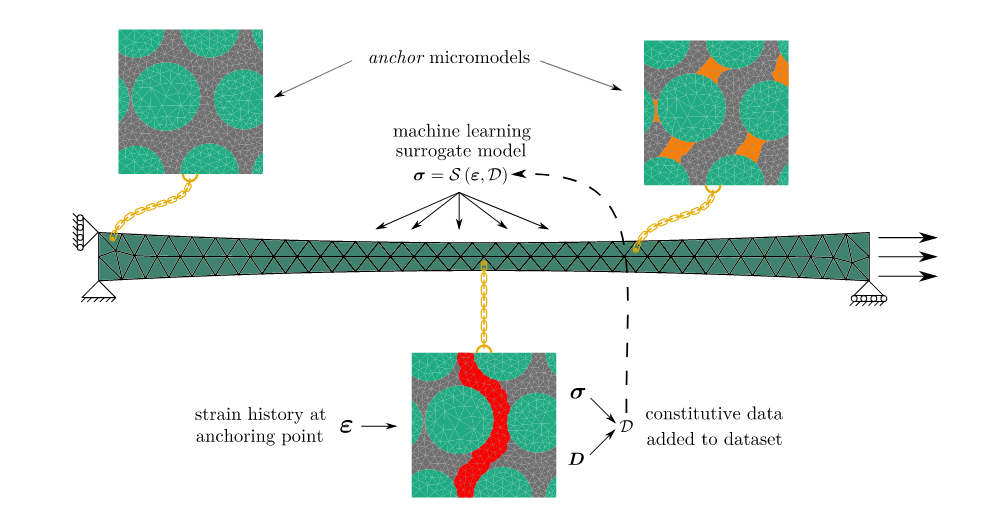
\includegraphics[width=1.1\textwidth]{Figures/anchor}
  \end{minipage}
\end{frame}

\begin{frame}{ML}
  \begin{minipage}{0.5\textwidth}
    \begin{itemize}
      \item Gaussian Process Regression with \textit{derivative} information.
      \item Application is 3-dimensional, but independent GP's are utilized.
    \end{itemize} 
  \end{minipage}%
  \begin{minipage}{0.5\textwidth}
    \centering
    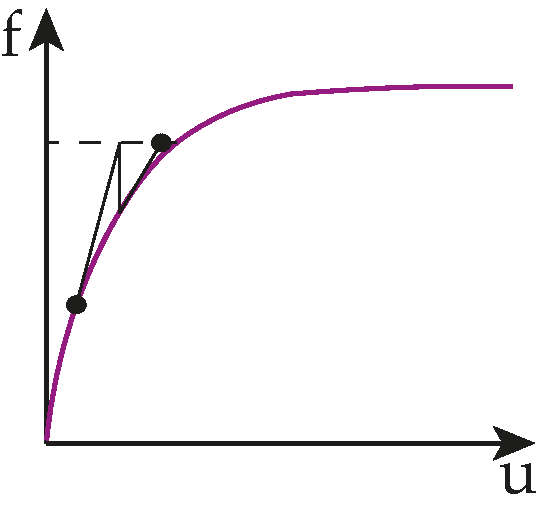
\includegraphics[width=0.8\textwidth]{Figures/nonlinear}
  \end{minipage}
\end{frame}

\begin{frame}{ML}
  \begin{minipage}{0.5\textwidth}
    \begin{itemize}
      \item Gaussian Process Regression with \textit{derivative} information.
      \item Use all data  to adjust the kernel hyper-parameters.
    \end{itemize} 
  \end{minipage}%
  \begin{minipage}{0.5\textwidth}
    \centering
    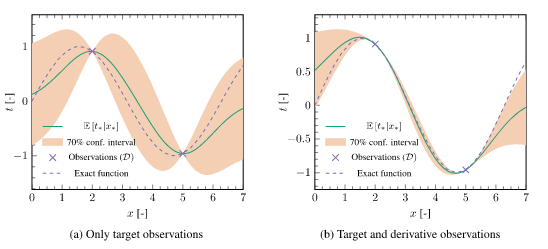
\includegraphics[width=1.1\textwidth]{Figures/gpr_deriv}
  \end{minipage}
\end{frame}

\begin{frame}{What is the main idea?}
  \begin{minipage}{0.5\textwidth}
    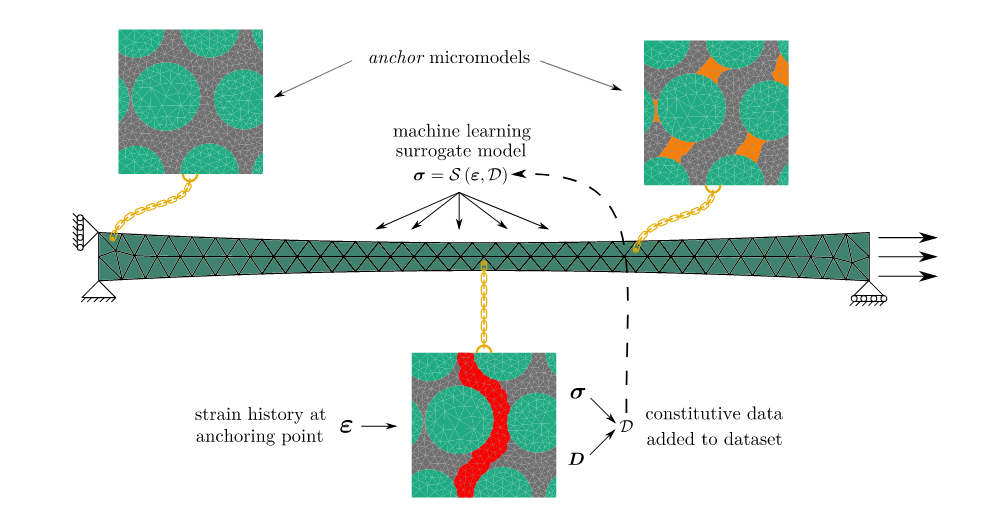
\includegraphics[width=1.1\textwidth]{Figures/anchor}
  \end{minipage}%
  \begin{minipage}{0.5\textwidth}
    \includegraphics<1>[width=1.1\textwidth]{Figures/heat}
    \begin{itemize}
      \item <1> Solve the simplest problem! 
      \item <1> With k-means clustering find anchor points
    \end{itemize}
  \end{minipage}
\end{frame}

\begin{frame}{What is the main idea?}
  \begin{minipage}{0.5\textwidth}
  \begin{itemize}
      \item <1> As you go along check your prediction variance
      \item <1>  $\gamma = \text{max}_i^3(\sqrt{\mathbb{V}[\sigma_i]})$
  \end{itemize}
  \end{minipage}%
  \begin{minipage}{0.5\textwidth}
    \includegraphics<1>[width=1.1\textwidth]{Figures/idea}
  \end{minipage}
\end{frame}

\begin{frame}{What is the main idea?}
  \begin{minipage}{0.5\textwidth}
  \begin{itemize}
      \item <1> As you go along check your prediction variance
      \item <1>  $\gamma = \text{max}_i^3(\sqrt{\mathbb{V}[\sigma_i]})$
  \end{itemize}
  \end{minipage}%
  \begin{minipage}{0.5\textwidth}
    \includegraphics<1>[width=1.1\textwidth]{Figures/observe}
  \end{minipage}
\end{frame}

\begin{frame}{Result-A}
  \begin{minipage}{0.5\textwidth}
    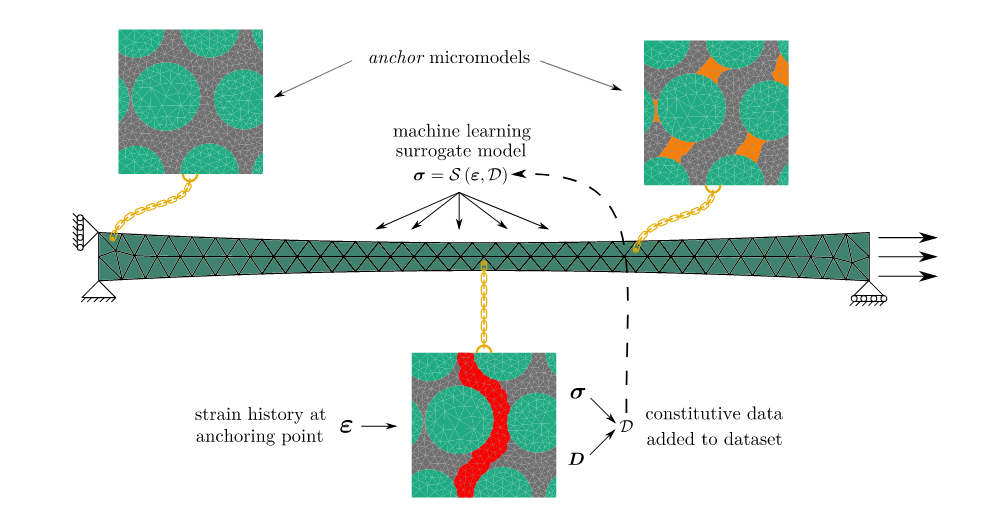
\includegraphics[width=1.1\textwidth]{Figures/anchor}
  \end{minipage}%
  \begin{minipage}{0.5\textwidth}
    \centering
    $\text{R}:= \frac{n_{\text{full}}}{n_{\text{gpr}}}$
    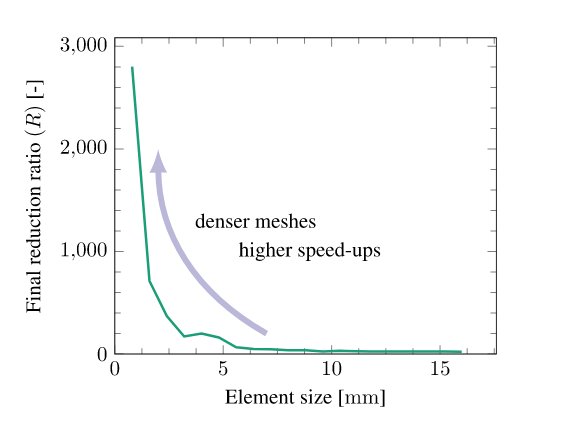
\includegraphics[width=1.1\textwidth]{Figures/result}
  \end{minipage}
\end{frame}

\begin{frame}{Conclusions}
  \begin{itemize}
    \item Speed ups with the combination of ml and direct numerical solvers 
    \item A bit fragile system as most of the information needed by the direct numerical solver comes from the surrogate models.
  \end{itemize}
\end{frame}

\begin{frame}
    \color{Pink} 
    \centering
     THANKS!
\end{frame}


\end{document}

